\subsection{求解结果}

\renewcommand{\arraystretch}{1.25}
\setlength{\LTpre}{6pt}
\setlength{\LTpost}{6pt}

我们采用Python调用SciPy/HiGHS线性规划求解器，基于上述模型利用附件2中365天的负载与光伏实测数据、附件1的电价曲线对全年购电计划进行求解，从2025年1月1日6000 kWh开始连续运行，结果统计区间为2月1日至12月31日，共334天，核心参数如表\ref{tab:参数2}所示。

\Needspace{0.30\textheight}
\begin{longtable}{>{\centering\arraybackslash}p{0.2244\textwidth}>{\centering\arraybackslash}p{0.2056\textwidth}>{\centering\arraybackslash}p{0.2244\textwidth}>{\centering\arraybackslash}p{0.2056\textwidth}}
  \caption{问题二全年运行汇总结果（2025-02-01 至 2025-12-31，共334天）}
  \label{tab:q2_sum} \\
  \toprule
  指标 & 数值 & 指标 & 数值 \\
  \midrule
  \endfirsthead
  \caption{问题二全年运行汇总结果（续）} \\
  \toprule
  指标 & 数值 & 指标 & 数值 \\
  \midrule
  \endhead
  \bottomrule
  \endfoot
  全年购电费（元） & 13790848.69 & 其中计划购电费（元） & 13322381.05 \\
  紧急购电费（元） & 468467.64 & 紧急购电费占比（\%） & 3.40 \\
  紧急购电量（kWh） & 75858.03 & 紧急购电日数（天） & 139 \\
  计划购电量（kWh） & 21748105.01 & 生效购电量（kWh） & 21748105.01 \\
  未消纳电量（kWh） & 2687529.82 & 计划执行偏差电量（kWh） & 0.00 \\
  2月1日初始储电量（1月预热后，kWh） & 9309.34 & 年末储电量（kWh） & 2233.58 \\
  LP求解失败次数 & 0 & 核查异常次数 & 0 \\
\end{longtable}

\begin{figure}[ht]
  \centering
  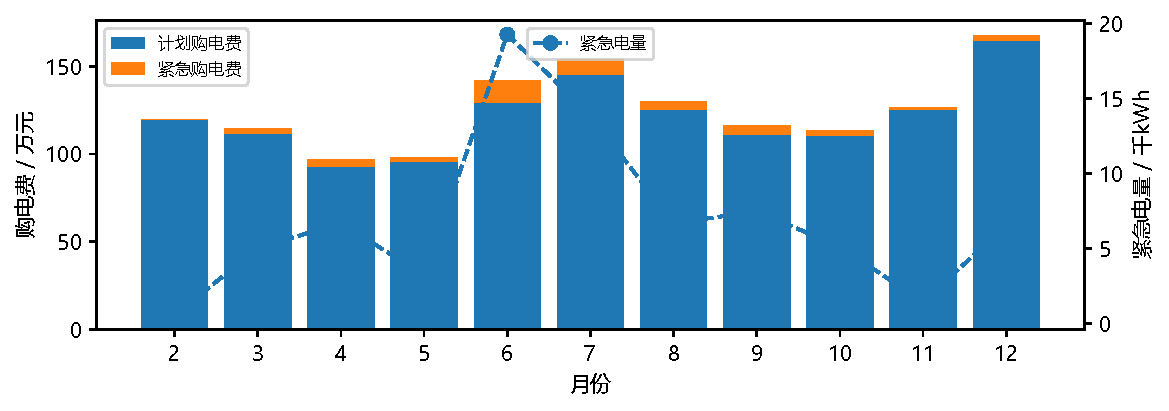
\includegraphics[width=0.86\textwidth]{figures/q2_month.pdf}
  \caption{月度购电费用构成与月度紧急购电量}
  \label{fig:q2_month}
\end{figure}

\begin{figure}[ht]
  \centering
  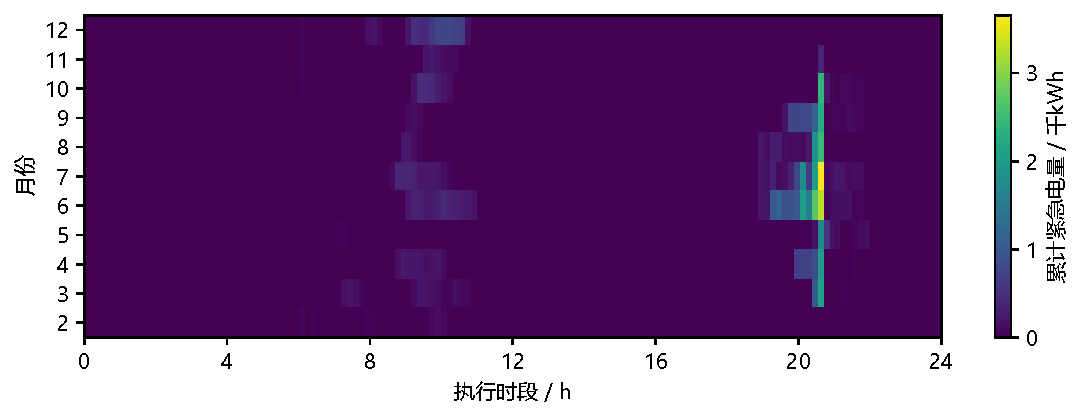
\includegraphics[width=0.94\textwidth]{figures/q2_heat.pdf}
  \caption{全年紧急购电量的月份—时刻分布热力图}
  \label{fig:q2_heat}
\end{figure}

\begingroup
\scriptsize
\setlength{\tabcolsep}{3pt}
\renewcommand{\arraystretch}{1.25}
\setlength{\LTpre}{6pt}
\setlength{\LTpost}{6pt}
\Needspace{0.30\textheight}
\begin{longtable}{>{\centering\arraybackslash}p{.18\textwidth}*{4}{>{\centering\arraybackslash}p{.18\textwidth}}}
\caption{问题二指定日期计划购电量及全天结果}\\
\toprule 时间段 & 2025.3.20 & 2025.6.21 & 2025.9.23 & 2025.12.21\\\midrule
\endfirsthead
\caption{问题二指定日期计划购电量及全天结果（续）}\\
\toprule 时间段 & 2025.3.20 & 2025.6.21 & 2025.9.23 & 2025.12.21\\\midrule\endhead
10:00--10:10 & 0.00 & 0.00 & 0.00 & 0.00\\
12:00--12:10 & 551.78 & 0.00 & 518.91 & 933.28\\
14:00--14:10 & 0.00 & 0.00 & 0.00 & 0.00\\
16:00--16:10 & 469.22 & 232.29 & 590.47 & 813.15\\
18:00--18:10 & 715.76 & 0.00 & 792.99 & 740.78\\
20:00--20:10 & 0.00 & 0.00 & 0.00 & 0.00\\
全天计划购电量/kWh & 63961.58 & 41564.93 & 71938.17 & 96584.50\\
全天购电费/元 & 40425.55 & 23144.61 & 44963.26 & 62257.10\\
\bottomrule
\end{longtable}
\begin{longtable}{>{\centering\arraybackslash}p{.18\textwidth}*{4}{>{\centering\arraybackslash}p{.18\textwidth}}}
\caption{问题二指定日期储能设备充放电量（kWh）}\\
\toprule 时间段 & 2025.3.20 & 2025.6.21 & 2025.9.23 & 2025.12.21\\\midrule
\endfirsthead
\caption{问题二指定日期储能设备充放电量（续，kWh）}\\
\toprule 时间段 & 2025.3.20 & 2025.6.21 & 2025.9.23 & 2025.12.21\\\midrule\endhead
0:00--4:00 & 1414.70/243.99 & 653.37/187.65 & 2130.19/22.43 & 1694.95/192.39\\
4:00--8:00 & 1030.64/4624.04 & 510.36/2101.65 & 237.88/5778.35 & 1288.87/1535.52\\
8:00--12:00 & 5874.89/2777.38 & 9321.76/0.00 & 5607.93/1896.62 & 5379.23/7222.74\\
12:00--16:00 & 3239.78/536.61 & 0.00/0.00 & 4035.26/553.40 & 7354.88/2258.56\\
16:00--20:00 & 276.97/5741.61 & 129.85/5635.54 & 288.28/5437.90 & 6.41/5593.78\\
20:00--24:00 & 4441.85/2884.47 & 8787.35/2514.82 & 8675.66/2915.06 & 8556.81/2842.53\\
0时/24时储电 & 9173.92/5149.20 & 3906.74/9769.51 & 8907.75/9336.82 & 9108.54/9133.22\\
\bottomrule
\end{longtable}
\begin{longtable}{>{\centering\arraybackslash}p{.24\textwidth}p{.40\textwidth}p{.20\textwidth}}
\caption{问题二指定日期紧急购电结果（kWh）}\\
\toprule 日期 & 紧急购电时间段 & 购电量\\\midrule
\endfirsthead
\caption{问题二指定日期紧急购电结果（续，kWh）}\\
\toprule 日期 & 紧急购电时间段 & 购电量\\\midrule\endhead
2025.3.20 & 20:30--20:40 & 89.36\\
2025.6.21 & 无 & 0.00\\
2025.9.23 & 20:20--20:30 & 6.38\\
2025.12.21 & 07:50--08:00 & 16.04\\
\bottomrule
\end{longtable}
\endgroup

